\documentclass[onecolumn, draftclsnofoot,10pt, compsoc]{IEEEtran}
\usepackage{graphicx}
\graphicspath{ {images/} }
\usepackage{url}
\usepackage{setspace}
\usepackage{float}
\usepackage{caption}
\setcounter{tocdepth}{3}
\usepackage{geometry}
\geometry{textheight=9.5in, textwidth=7in}
\usepackage{listings}

% Taken from http://timmurphy.org/2014/01/27/displaying-code-in-latex-documents/ with some modifications
\lstset{
    frame=none,
    tabsize=4, % tab space width
    showstringspaces=false, % don't mark spaces in strings
    numbers=none, 
    commentstyle=\color{green}, % comment color
    keywordstyle=\color{blue}, % keyword color
    stringstyle=\color{red}, % string color
    basicstyle={\small\ttfamily}, % font style
    belowcaptionskip=1\baselineskip
}

% 1. Fill in these details
\def \CapstoneTeamName{		Skill Capped IRL}
\def \CapstoneTeamNumber{		17}
\def \GroupMemberOne{			Katherine Bajno}
\def \GroupMemberTwo{			Meagan Olsen}
\def \GroupMemberThree{			William Sims}
\def \GroupMemberFour{			Kiarash Teymoury}
\def \CapstoneProjectName{		eBay iOS eSports Application}
\def \CapstoneSponsorCompany{	eBay}
\def \CapstoneSponsorPerson{		Luther Boorn}

% 2. Uncomment the appropriate line below so that the document type works
\def \DocType{		%Problem Statement
				%Requirements Document
				%Technology Review
				Design Document
				%Progress Report
				}
			
\newcommand{\NameSigPair}[1]{\par
\makebox[2.75in][r]{#1} \hfil 	\makebox[3.25in]{\makebox[2.25in]{\hrulefill} \hfill		\makebox[.75in]{\hrulefill}}
\par\vspace{-12pt} \textit{\tiny\noindent
\makebox[2.75in]{} \hfil		\makebox[3.25in]{\makebox[2.25in][r]{Signature} \hfill	\makebox[.75in][r]{Date}}}}
% 3. If the document is not to be signed, uncomment the RENEWcommand below
%\renewcommand{\NameSigPair}[1]{#1}

%%%%%%%%%%%%%%%%%%%%%%%%%%%%%%%%%%%%%%%
\begin{document}
\begin{titlepage}
    \pagenumbering{gobble}
    \begin{singlespace}
    	% Need to uncomment this line below to include the COE photo
    	%
\includegraphics[height=4cm]{coe_v_spot1}
        \hfill 
        % 4. If you have a logo, use this includegraphics command to put it on the coversheet.
        %\includegraphics[height=4cm]{CompanyLogo}   
        \par\vspace{.2in}
        \centering
        \scshape{
            \huge CS Capstone \DocType \par
            {\large\today}\par   
            \vspace{.5in}
            \textbf{\Huge\CapstoneProjectName}\par
            {\large CS461 Senior Software Engineering Project I}\par
            {\large Fall 2017}\par
            \vfill
            {\large Prepared for}\par
            \Huge \CapstoneSponsorCompany\par
            \vspace{5pt}
            {\Large\NameSigPair{\CapstoneSponsorPerson}\par}
            {\large Prepared by }\par
            Group\CapstoneTeamNumber\par
            % 5. comment out the line below this one if you do not wish to name your team
            \CapstoneTeamName\par 
            \vspace{5pt}
            {\Large
                \NameSigPair{\GroupMemberOne}\par
                \NameSigPair{\GroupMemberTwo}\par
                \NameSigPair{\GroupMemberThree}\par
                 \NameSigPair{\GroupMemberFour}\par
            }
            \vspace{20pt}
        }
        \begin{abstract}
        % 6. Fill in your abstract
This purpose of this document is to create a roadmap of the steps we will take to develop the eBay iOS eSports application. 
The designs for various components of the application are described in detail and analyzed from different viewpoints.
Also outlined is the software architecture and user interface design that will be implemented. 
            
        	%This document is written using one sentence per line.
        	%This allows you to have sensible diffs when you use \LaTeX with version control, as well as giving a quick visual test to see if sentences are too short/long.
        	%If you have questions, ``The Not So Short Guide to LaTeX'' is a great resource (\url{https://tobi.oetiker.ch/lshort/lshort.pdf})
        \end{abstract}     
    \end{singlespace}
\end{titlepage}
\newpage
\pagenumbering{arabic}
\tableofcontents
% 7. uncomment this (if applicable). Consider adding a page break.
%\listoffigures
%\listoftables
\clearpage

% 8. now you write!

\section{Introduction}

\subsection{Scope}
Our main goal is to create an application that helps eBay learn more about the eSports market and new shopping opportunities for eBay. The software will allow users to find and purchase eSports merchandise that is being sold on eBay. We also want to create an environment for millennial gamers to learn more about upcoming eSports events around the world. This project will be developed between December of 2017 and May of 2018.

\subsection{Purpose}
This document outlines the details of how the eBay iOS eSports Application will be structured. It provides in-depth details about the design including a conceptual model and a design description including viewpoints, languages, and influences.

\subsection{Intended audience}
The intended audience for this document is Luther Boorn and the mentors from eBay including Steve Splonskowski, Silas Marshall, Darrekk Hocking, and Brandon Lee. It is also intended for the instructors of the Capstone course, Kevin McGrath and Kirsten Winters. 

\subsection{Conformance}
The eBay iOS eSports application will conform to the requirements as detailed in sections four and five of this document and the specifications provided by the client. The previously mentioned sections can be referenced for more specifications on the application requirements and conformance.

\section{Definitions}

\begin{itemize}

\item \textbf{Client:} Luther Boorn, eBay
\item \textbf{JSON:} JSON or JavaScript Object Notation, is an open-standard file format that uses human-readable text to transmit data objects consisting of attribute–value pairs and array data types.
\item \textbf{UI:} UI or user interface, is the space where interactions between humans and machines occur.
\item \textbf{API:} API or application programming interface, is a set of subroutine definitions, protocols, and tools for building application software.
\item \textbf{MVC:} Model-view-controller (MVC) is a software architectural pattern for implementing user interfaces on computers.
\item \textbf{Firebase:} Real time database service provided by Google which offers cloud messaging, storage, and authentication.
\item \textbf{Swift:} Compile programming language provided by Apple to build application for the iOS and Mac OS X.
\item \textbf{Xcode:} IDE provided by Apple to test, compile and develop applications for the iOS and Mac OS X.
\item \textbf{eSports:} Multiplayer gaming event thats played competitively through out the world among professional gamers.
\item \textbf{iOS:} Mobile operating system created and developed by Apple. 

\end{itemize}

\section{Conceptual model for software design descriptions}
This section contains the conceptual model for the eBay eSports iOS application design. 
Included are basic terms and concepts of the software design descriptions, the context in which software design descriptions are prepared and used, the stakeholders who use them, and how they are used.

\subsection{Software design in context}
The application will be designed using object-oriented programming and the model-view-controller (MVC) design pattern. 
In context, our models, views, and controllers will be implemented using Swift. 
The model will retrieve data stored in Firebase and send it to the controller which will update the view accordingly\cite{fb}. 
Data will also be retrieved by calling the Twitter API and eBay Browse API. The returned JSON data will be converted to Swift data types and objects that represent the business logic of our application. Model data will be communicated to the view using the controller. 
Views will be implemented using the Apple UIKit which provides the window and view architecture for implementing the interface.
User data such as login information and favorites will be written to the Firebase database. 
\begin{figure}[H]
\centering
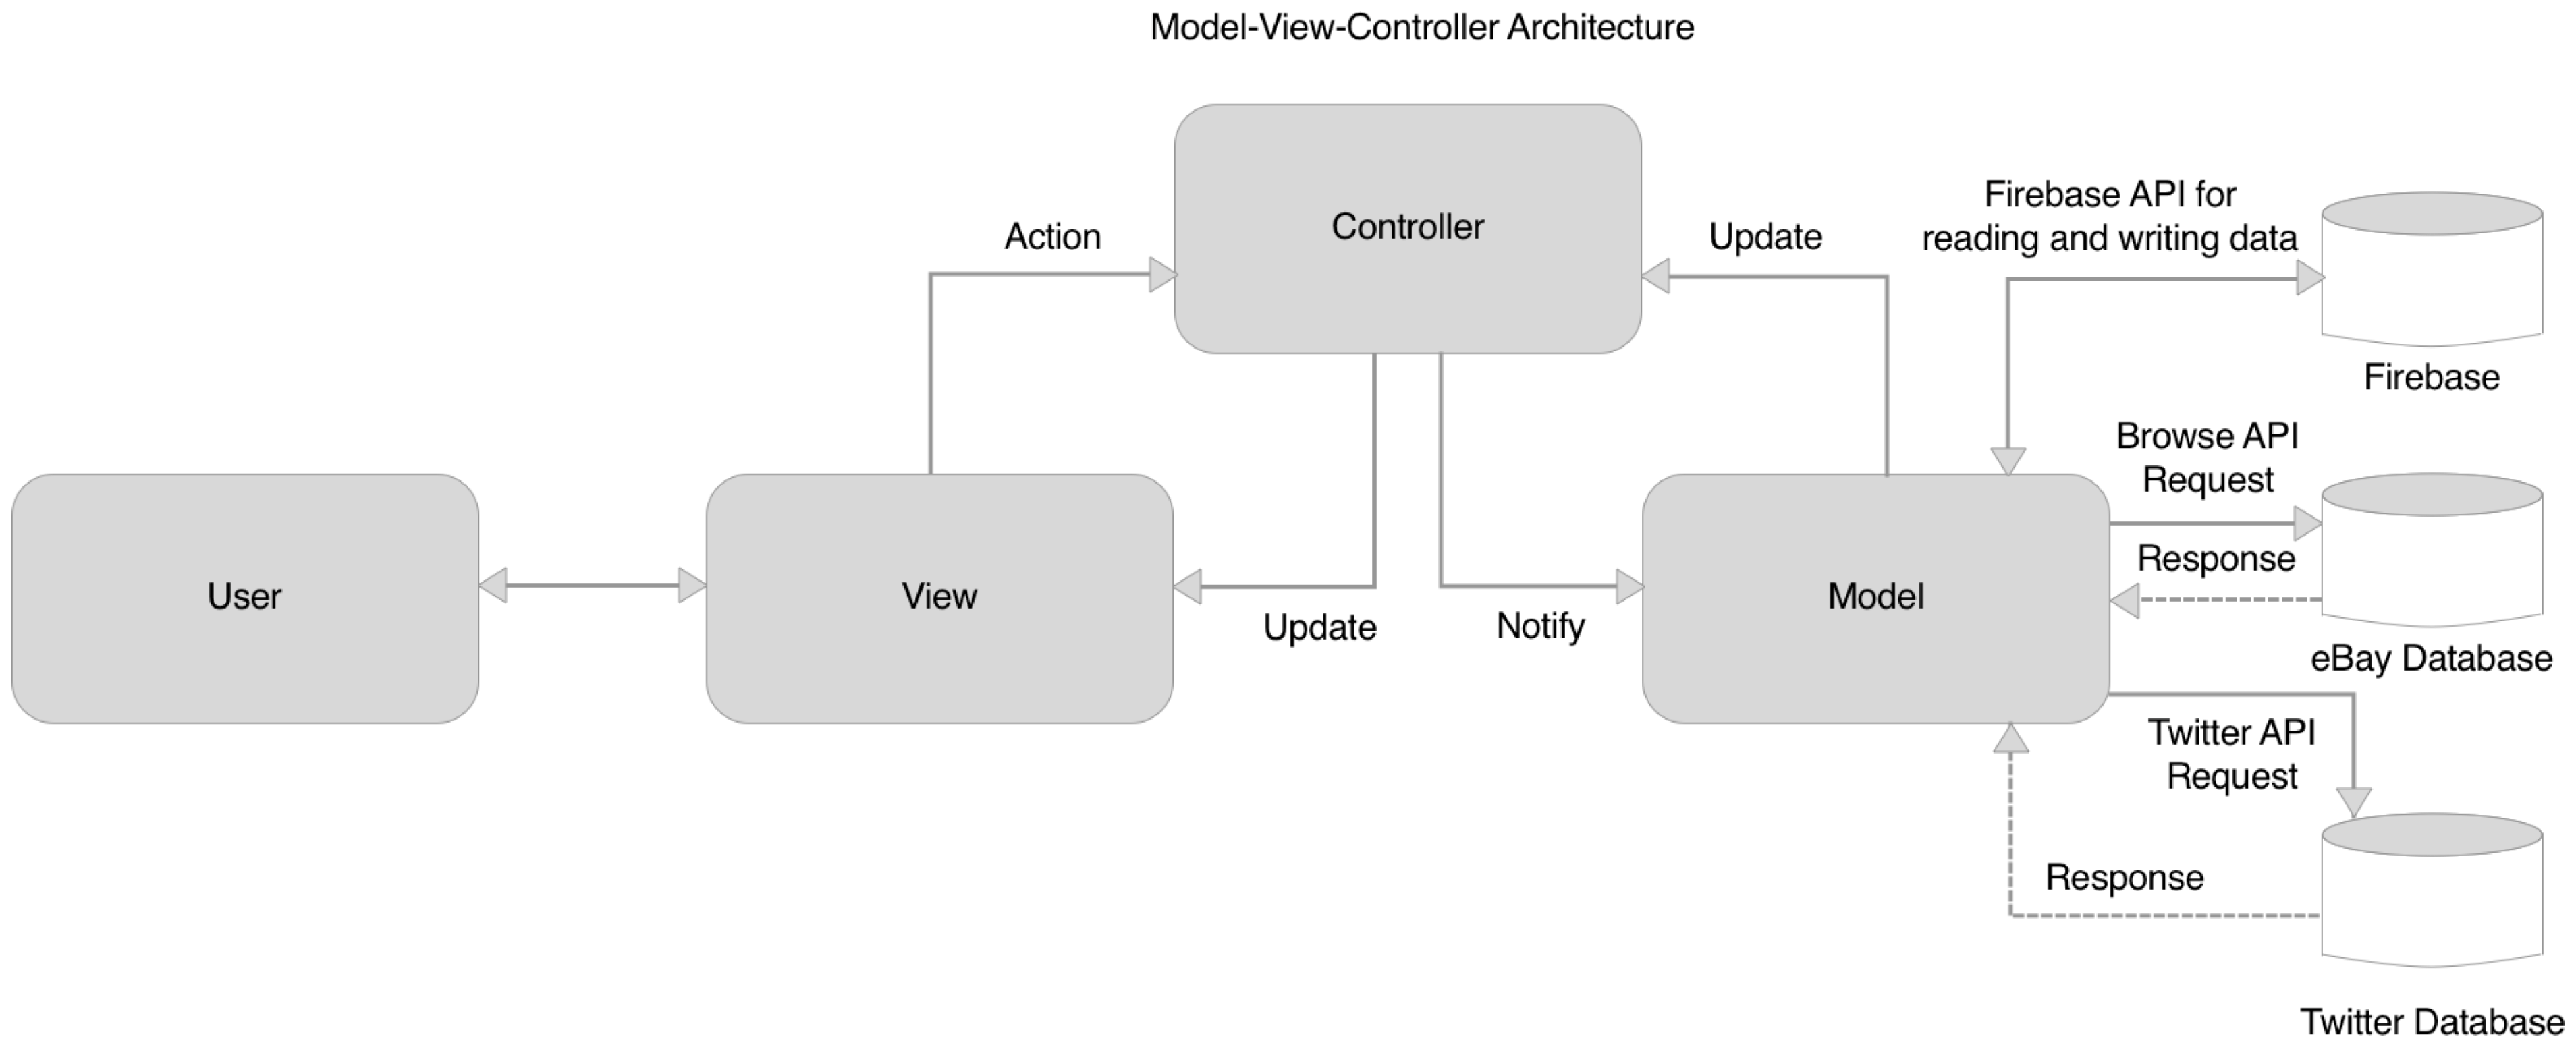
\includegraphics[scale=.20]{MVC}
\caption{Diagram of Model-View-Controller Design}
\end{figure}

\subsection{Software design descriptions within the life cycle}
 
\subsubsection{Influences on SDD preparation}
The design of our application is driven by our software requirements specification. 
The requirements outline the functionality desired by our client and directly impact how we plan to implement the application.
\subsubsection{Influences on software life cycle products}
The software life cycle of our application will be influenced primarily by the requirements document. Retrieving and storing data from APIs will be very important to successfully complete the project objectives. 
Therefore, data collection and storage will be implemented first in the software life cycle. 
The next step in the software life cycle will involve manipulating and displaying the data in a way that matches client specifications.
\subsubsection{Design verification and design role in validation}
Verification of whether our application fulfills specified requirements will be done through unit tests and client verification.
Data returned from API calls will be checked to ensure that the correct information was received before updating relevant models.
JSON data that has been received and converted in Swift data types will be tested for correctness. Unit tests will be implemented throughout the development life cycle to make certain that our project requirements are being met. 

\section{Design description information content}

\subsection{Introduction}
This section outlines details about the different components that went into creating the overall design. The details include information about the design stakeholders, design views, design viewpoints, design elements, design entities, design attributes, design relationships and constraints, the design rationale, and the design language.

\subsection{Design stakeholders and their concerns}
The stakeholders of this project are from eBay and include Luther Boorn, Steve Splonskowski, Silas Marshall, Darrekk Hocking, and Brandon Lee. Their concern entails the application being completed with the discussed features. Another concern is for the application to be built in such a way that new upcoming eSports events, games, and teams can be easily introduced.

\subsection{Design views}
The design views will utilize a MVC structure. This will allow the application to address the design concerns posed by the client. By categorizing the application into the model, view, and controller sections, it allows us to focus on the design in specific perspectives. The model section includes our data including user and game information, the view's will represent the UI implemented using the Apple UIKit, and the controller will represent the information being sent between the model and view.

\subsection{Design viewpoints}
This section details the viewpoints that are discussed in section five pertaining to the design of the components of the eBay iOS eSports application. These viewpoints include the pattern viewpoint, resources viewpoint, dependency viewpoint, context viewpoint, interface viewpoint, and the interaction viewpoint.

\subsubsection{Pattern Viewpoint}
When developing the eBay iOS eSports application, many elements will be reusable and repeatable. This is to ensure that the individuals using this software will find information on the application consistent and intuitive. By repeating the same page layout on the various activities in the application, the code structure becomes reusable.

\subsubsection{Resources Viewpoint}
The application relies on various resources including the Twitter API, eBay Browse API, and Firebase. These resources are a part of the back-end of the application. Data will be stored and retrieved from them.

\subsubsection{Dependency Viewpoint}
While each section of the application is an independent component, they are dependent on one another to some extent. This follows the MVC model being implemented. User functions in the application such as signing in, viewing favorites, viewing merchandise, and browsing games are all depended on the data stored in the Firebase and retrieved from the eBay Browse API properly being sent by the controller to the UI view.

\subsubsection{Context Viewpoint}
The components and user features of the application must satisfy the client's concerns. The UI should be simple and intuitive for the user to interact with. The user should be able to complete all actions using touch, and should not require a high-level understand of technology.

\subsubsection{Interface Viewpoint}
The UI is essential to this application. The interface should display all information for the user including games, events, tweets, favorites, and merchandise. The user will interact with the interface through touch, and will be able to control it to an extent by favoring items and having them display on their home page when logged in.

\subsubsection{Interaction Viewpoint}
Each component of the application must interact with one another for the application to work as intended. In the MVC model, this is the job of the controller to be the connection for the data stored in the model and the UI view to interact. The interaction details of each component are explained in section five.

\subsection{Design rationale}
The design was discussed between the client and team members of Skill Capped IRL to decide what best met the specifications for both the user and the application. The choices were made with the user in mind including factors such as ease of use and intuitiveness. Various elements of the design may adjust as the development happens if the original design is not the best for the user.

\subsection{Design languages}
After the designs were discussed, the Max OSX program Sketch was used to visualize the design. The various application activity screens layouts were created using this program.

\section{Design viewpoints}

\subsection{Introduction}
This section outlines various design components using various viewpoints. The design components discussed include developing the user interface, data storage, user authentication, the user interface design, networking, the Twitter API, and the eBay Browse API. The viewpoints in which they are discussed include the pattern viewpoint, resources viewpoint, dependency viewpoint, context viewpoint, logical viewpoint, information viewpoint, interface viewpoint, and interaction viewpoint.

\subsection{Developing the User Interface}
The user interface will be developed using custom code rather than storyboards or xibs. Doing it this helps avoids the problems of the complexity, possibility of too large of storyboards, and the merge conflicts that can arise from them with four different developers working on the same thing.While this may create more of a challenge visually, it also provides more freedom for more custom, dynamic layouts than storyboards or xibs. Using custom code will help provide us as developers a better understanding of the user interface that can be overlooked when using xibs and storyboards.  
 \subsubsection{Pattern Viewpoint}
  From a pattern viewpoint, using custom code will present an advantage for replicating views as storyboards and templates do not allow for things like inheritance. While it is possible to create duplicate storyboards or xibs, these duplicate views are then separate from the original.
  \subsubsection{Resources Viewpoint}
  From a resources viewpoint, using custom code will help bypass the performance drain that comes with using xibs and storyboards. Because xibs and storyboards have to be loaded and parsed, this creates a performance overhead that is not found when the UI is coded from scratch. 
  \subsubsection{Dependency Viewpoint}
  Testing the user interface will depend on both the correct implementation of the back end data storage, meaning that the database is correctly storing the right data. Once the application is complete, testing functionality in the user interface will also rely on correct data binding between the back end database and the views. This data binding is discussed in the topic of networking. 
   \subsubsection{Context Viewpoint}
   From the perspective of the users, millennial gamers will have an assumed  knowledge of the different types of eSports games and the way that they are scored. Therefore, the user interface will contain intuitive elements and functionality that is familiar and pleasing to this interface's audience.
   
\subsection{Firebase Data Storage}
\subsubsection{Context Viewpoint}
Firebase is used to allow our users to sign up and log in to create a bridge between the application and the backend storage. Data will be written to Firebase database to allow an interaction between the users and data being passed around. Since Firebase is a real-time database, any changes made by the user will instantly update the user interface.

\subsubsection{Logical Viewpoint}
Every user receives a user id from Firebase after they fully get authenticated. This way we are able to easily write and parse JSON data retrieved from the database using queries.

\subsubsection{Dependency Viewpoint}
Since Firebase is offered by Google, they make updates pretty regularly to make it more stable and reliable. Currently, Firebase SDK is fully updated to support Swift 4 and it includes everything needed to create an interaction between the backend and the application.
\subsubsection{Information Viewpoint}
There are essentially there important methods that the Firebase SDK includes to allow us to write, retrieve, check for update.
\begin{lstlisting}
db.collection("Users")
\end{lstlisting}
Every call will include this method to do either of the three things mentioned. "db" is just our variable that is an instant of Firestore.firestore()  which includes the collection method. "Collection" is another term for the entity that we are trying to access from the data storage. \\
\noindent\textbf{Updating and writing to the database}
\begin{lstlisting}
.addDocument(data: user.infoDic) { error in
\end{lstlisting}
For writing to the database, we have to use a dictionary to have set of keys and values which in the database will be our attribute with their given value.

\noindent\textbf{Retrieving Data}
\begin{lstlisting}
.getDocuments() { querySnapshot, error in 
\end{lstlisting}
getDocument will return everything that is included in the user attribute. 

\noindent\textbf{Checking for changes in the database}
\begin{lstlisting}
.whereField("Name", isEqualTo: "Kia").addSnapshotListener { querySnapshot, error in 
\end{lstlisting}

\noindent "whereField" is another method provided by "collection" that is used to query specific attributes. All these methods eventually give us a completionHandler that contains the querySnapshot and the possible error object that we could use for error handling to avoid possible crashes.
\subsubsection{Interface Viewpoint}
In the context of this application, we are only using Firebase to update our user's favorited games. Therefore, the only things being changed on the main UI is the list of all the games that user has favorited. 
\subsubsection{Interaction Viewpoint}
The only interaction the user will have with the database is to be able to update their information and most importantly be able to favorite and unfavorite games.
\subsection{Firebase User Authentication}
\subsubsection{Context Viewpoint}
The user authentication will take place using Firebase authentication. Firebase authentication has the advantage of providing some built in resources that are easy to implement including SDKs and pre-built libraries. Firebase authentication supports a wide variety of application mediums including websites and mobile devices. It also catches many edge cases that could turn in security vulnerabilities which might introduce malicious material into the application if not caught. This authentication  supports many different forms of authentication including UI authentication and SDK authentication. This authentication choice integrates well with the back end data storage.
\subsubsection{Composition Viewpoint}
From a composition viewpoint, Firebase UI has the option of incorporating authentication from a variety of different sources including phone, email, Facebook, Twitter, and Google.The Firebase UI is composed of the Firebase Authentication SDK. Each of the views has a listener which keeps track of sign in state. This listener has methods which support signing up a user, retrieving information and profile about a user, signing in a user, and other functions relating to managing a user. This application chooses to use the custom password and username accounts, so it also has support for setting up those accounts and signing in with the created accounts.
\subsubsection{Dependency Viewpoint}
From a dependency viewpoint,the Firebase SDK must be installed and initialized. In addition, the support for each of the functions above requires that Firebase be first imported into the actual iOS application. It also necessary to attach the listeners to the relevant views in the application. 

\subsection{Twitter API}
The Twitter Kit for iOS will be used to retrieve Twitter data for our application by making REST API calls\cite{twitter}. 
Tweets from accounts relevant to the event featured on the home screen will be displayed. 
\subsubsection{Context Viewpoint}
The user will be able to view tweets that are related to the content being displayed on the home screen. The tweets will provide information about eSports events and improve user engagement. Tweets that contain profanity will be filtered out to provide an experience that is appropriate for all ages. The context of the tweets will pertain to the featured event to ensure that useful information is displayed. 
\subsubsection{Logical Viewpoint}
The Twitter API returns JSON data that will be converted into Swift data types using the JSONSerialization class included with the default Apple Foundation Framework\cite{json}. 
A model definition for Tweets will be created in order to store the data in Swift objects. 
The general method for converting JSON to Swift data types can be applied to data returned from Firebase and the eBay Browse API.
\subsubsection{Dependency Viewpoint}
The Twitter Kit for iOS has been updated for Swift 4 and can easily be installed with the most recent version of CocoaPods. 
The UI components that are part of the Twitter SDK have also been updated and are currently stable. 
\subsubsection{Information Viewpoint}
GET statuses/user\_timeline will be the primary API call that will be used to retrieve tweets from targeted accounts. 
The call returns a collection of the most recent tweets posted by the user indicated by the screen\_name or user\_id parameters. 
The screen name, text, date created, image URL, and profile image URL JSON values will be used to display the tweets in the user interface. 
\subsubsection{Interface Viewpoint}
The Twitter Kit for iOS includes built in components for displaying tweets in the user interface. 
Once a tweet has been loaded from network, a view will be created using the Twitter model object.
The TWTRTweetViewStyleCompact style will be used for displaying the tweets.
Retweets and favorites will not be displayed in the compact view style. 
\subsubsection{Interaction Viewpoint}
The user will not be able to favorite, modify, or delete Tweets displayed in the interface.
The compact view will display the user screen name, Twitter handle, date, text, profile image, and tweet image if applicable. The user will not directly interact with the tweets and the content will be displayed as a static image. 

\subsection{eBay Browse API}
\subsubsection{Context Viewpoint}
The eBay browse API is essential for this application. This application will be making calls to retrieve related merch related to each game. The data parsed will then be displayed to the user will all the item information. 

\subsubsection{Logical Viewpoint}
The application will make GET calls to the browser API to give us data object back. Then using apple JSONSerialization class which is included in the Apple SDK, we could parse each object and update our main UI. 

\subsubsection{Dependency Viewpoint}
This is the beta release of eBays browse API. Since they are not providing any SDKs then we don't have to worry about it is fully compatible with our application. The application is using apples URLSession class to make calls and retrieve data. Therefore, it will always be updated if there are any updates to the iOS SDK. 

\subsubsection{Information Viewpoint}
Search for Items by Keyword will be used by making a GET request to retrieve data

\begin{verbatim}
GET /item_summary/search
https://api.ebay.com/buy/browse/v1/item_summary/search?q="Leage+of+Legends&limit=3
\end{verbatim}
making a call to the API using URLSession() object
\begin{verbatim}
let keyWord: String
let FetchLimit: Int
if let baseURL = URL(string: "https://api.ebay.com/buy/browse/v1/item_summary/search?q=\(keyWord)&\(FetchLimit)") {
    URLSession().dataTask(with: baseURL!) {
        (data, response, error ) in
        if error != nil {
            //Error Handling
            return
        }
        
    //Parse JSON
    }.resume
}
\end{verbatim}

\noindent Using this query we could fetch 3 different merchandise that is associated with "League of Legends". This will return us a JSON with an array of different items. Each Item will have its own ID and attributes that would use to display item information on the main UI.
\subsubsection{Interface Viewpoint}
Our UI is one of the most important components, we are updating each UI element that is associated with the merchandise. The application will show the price, name and other details regarding the item.
\subsubsection{Interaction Viewpoint}
The fetched data will be displayed on our browse page where players get to see all the different merchandise populated with the items. As soon as the user clicks on one of the items, we will then display all the items details using the parsed JSON. 
\subsection{User Interface Design}

\subsubsection{Context Viewpoint}
    The user interface design entails the design of a user interface for the eBay iOS eSports mobile application. The interface will conform to the Apple iOS Human Interface guidelines. This application will be designed in such a way that each page has its own view, and this section details these views and how they are connected.\\
     \indent\textbf{Design Elements and Entities}
     \begin{itemize}
     \item Actors
       \begin{itemize}
       \item eSports fans 
        \end{itemize}
       
     \item Services
      \begin{itemize}
      \item query for an item
      \item filter which type of merchandise appears on the screen after a search 
      \item view information about a particular item 
      \item view relevant items to upcoming eSports events
      \item display eSports merchandise
      \item favorite games
      \item view favorites
      \item view information about a particular game 
      \item sign in
      \item register 
      \item view twitter feeds for games
      \item browse items by events, games, or teams
       \end{itemize}
       \end{itemize}
       
       \textbf{Design Relationships}
       \begin{itemize}
       \item The user will query for an item by selecting which game, event, or possibly team that they want to view items for.
       \item The user will filter for which type of merchandise they want want, by selecting from a drop down menu which type of merchandise they wish to view.
       \item The user will view information about a particular item by selecting the desired item from the list of items that appear on the page. 
       \item The user will view relevant items to upcoming eSports events by navigating to the event page.
        \item The user will display eSports merchandise by selecting which type of eSports topic they want to search by and filtering which type of merchandise they want.
        \item The user will view favorites by signing in and navigating to the home page.
        \item The user will view information about a particular game by clicking on the event from the home page. 
        \item The user will sign in by entering their user credentials on the sign in page. 
        \item The user will register by entering their information on the register page. 
        \item The user will view twitter feeds for games by clicking on the twitter feed from the home page. 
        \item The user will browse items by selecting which category they want to search by. 
        \end{itemize}
         
        \subsubsection{Dependency Viewpoint}
        The user interface is dependent on the networking from the back end Firebase Database to the views. The UI displays the data while the networking grabs the data from the database.
        \textbf{Design Concerns}
        The UI will be divided into the following pages:
       \begin{itemize}
       \item home page-displays favorites, twitter feeds, 
       \item event page-displays eSports merchandise, rel event information and twitter feeds 
       \item twitter feeds page-displays twitter feeds for a category
       \item register-allows user to register
       \item login page -allows user to login 
       \end{itemize}
       \textbf{Design Relationships}
       \begin{itemize} 
       \item The home page relies on all other pages since it provides links to all of them. 
       \item The event page relies on the home page since the user navigates to the event page via the home page. 
       \item The twitter feeds page relies on the home page as a specific game has to be selected.
       \item The register page relies on the home page as the home page allows the user to register for an account 
       \item The sign in page is the first page, but it relies on the user first visiting the register page.
       \end{itemize}
   \subsubsection{Interface Viewpoint}
          \begin {itemize}
          \item The home page must have as an input valid user credentials after a user is signed in and outputs navigation to all other pages.
          \item The event page takes as an input a particular event and outputs information about that event as well as merchandise and relevant tweets.
          \item The twitter feeds page takes in as an input the game or event describing the feeds and outputs the list of feeds. 
          \item The register page inputs a username and password for the account being set up.
          \item The sign in page takes the username and password of the account being accessed and outputs the corresponding home screen or an error message if valid credentials cannot be found.
          \end {itemize} 
          
\begin{figure}[H]
\centering
\captionsetup{justification=centering}
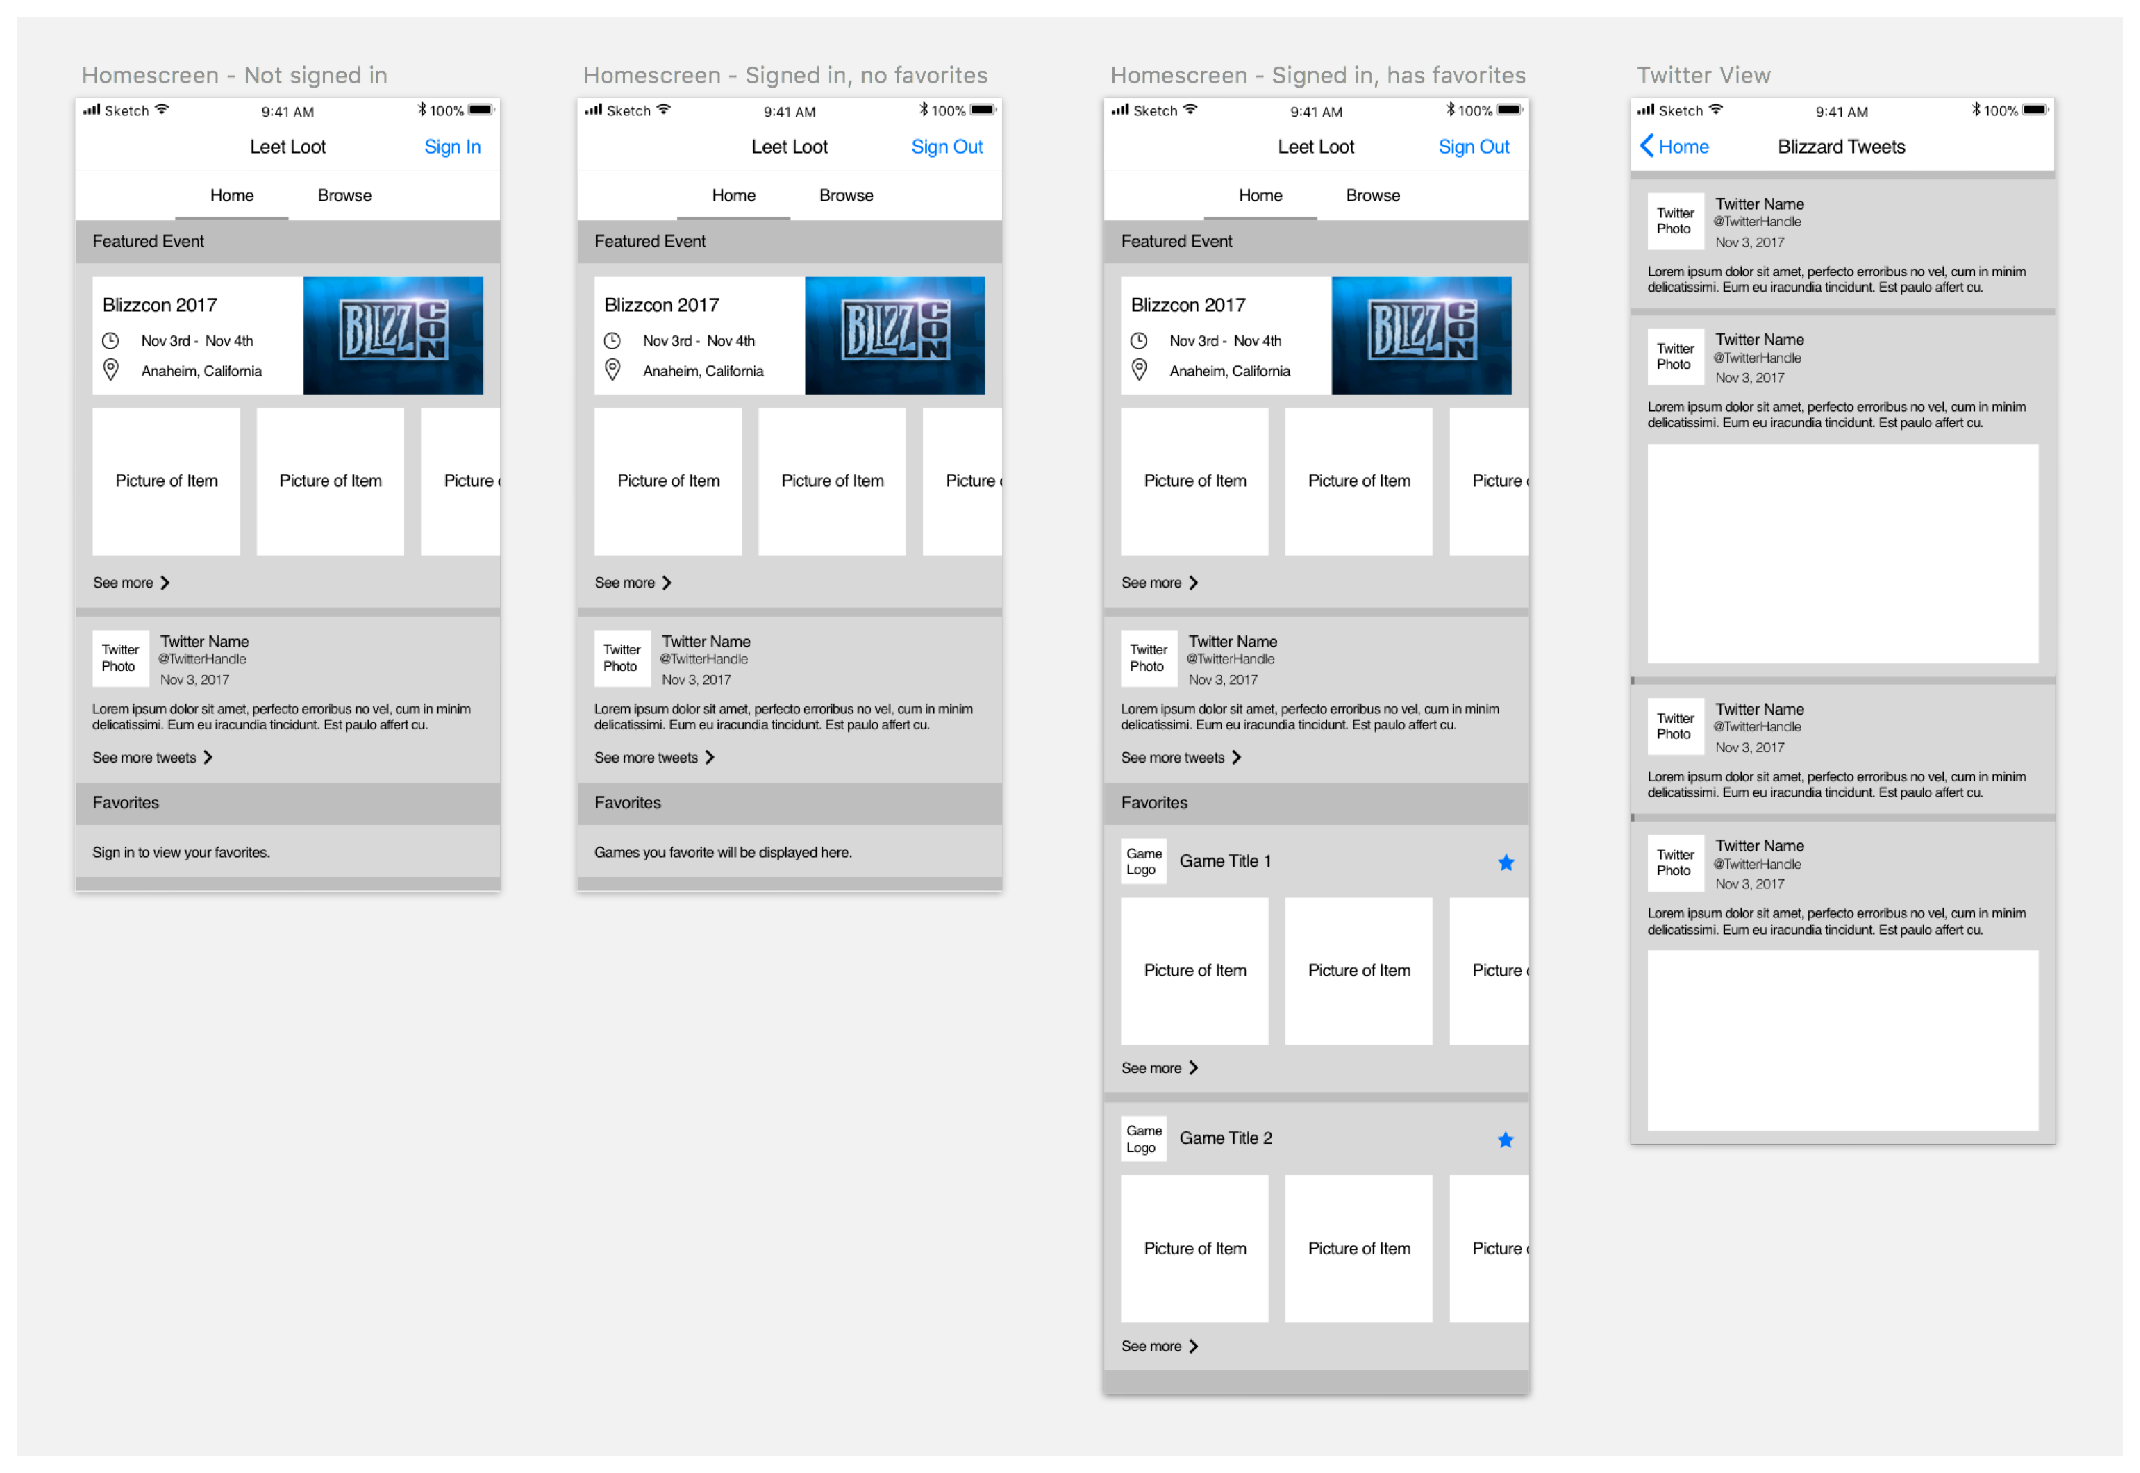
\includegraphics[scale=.50]{Homescreen}
\caption{Home screen User Interface}
\end{figure}

\begin{figure}[H]
\centering
\captionsetup{justification=centering}
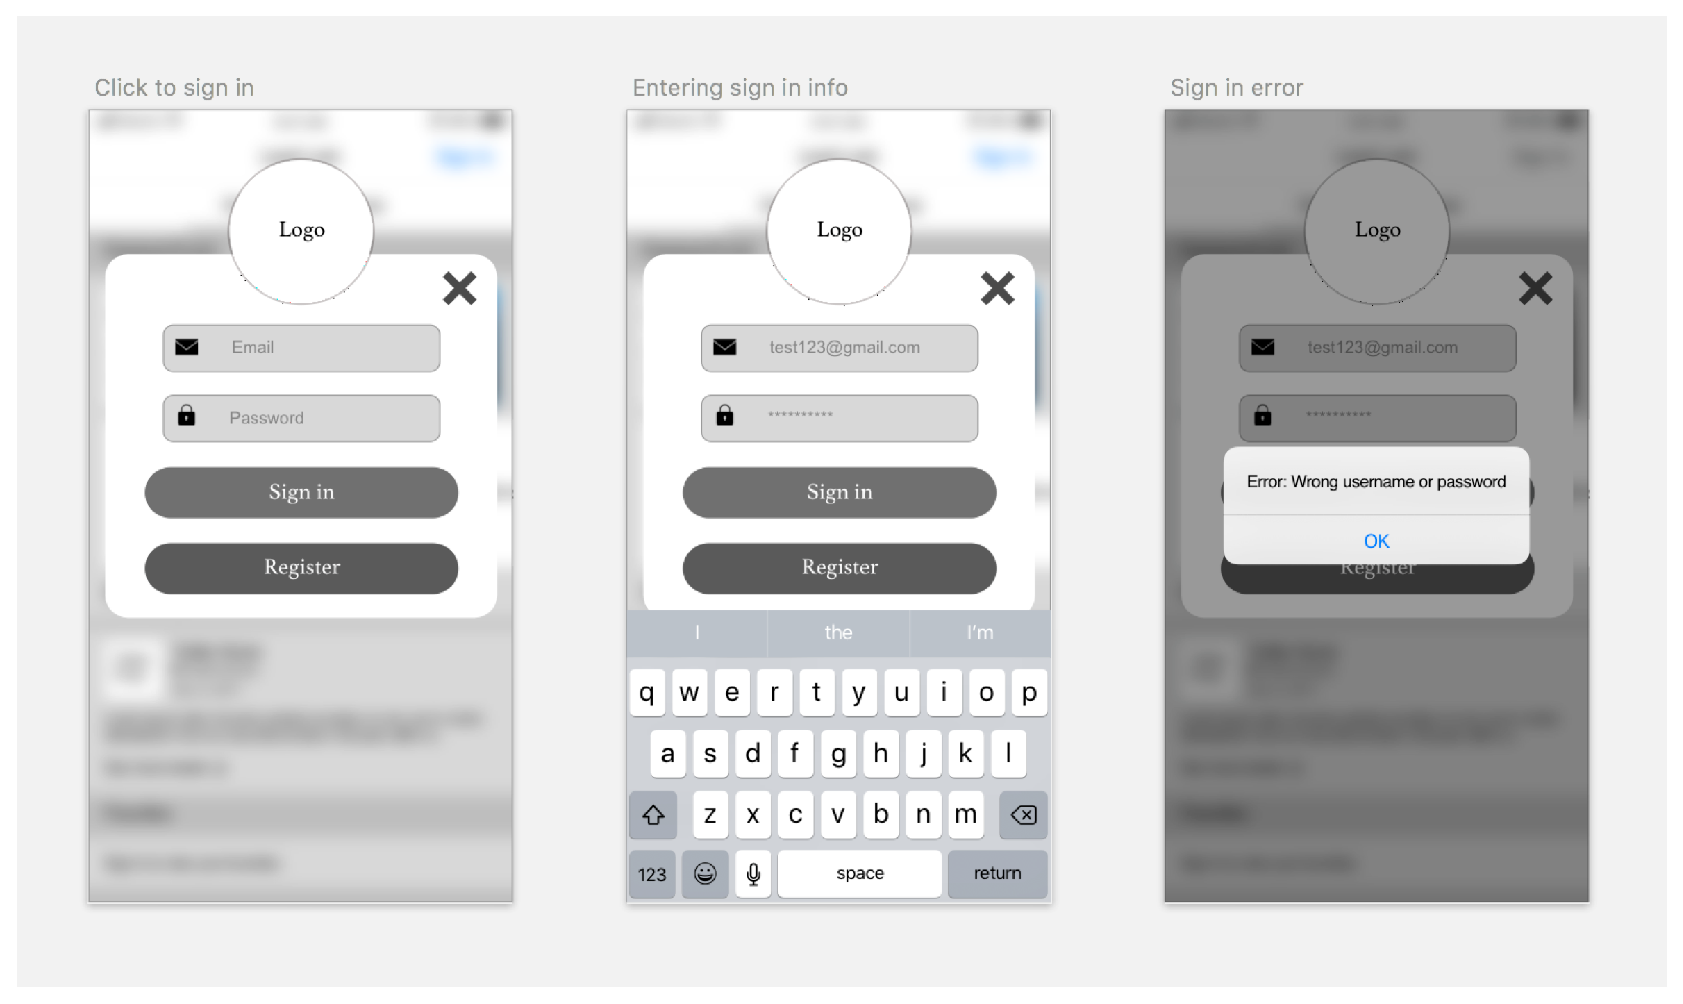
\includegraphics[scale=.50]{SignIn}
\caption{Sign In User Interface}
\end{figure}

\begin{figure}[H]
\centering
\captionsetup{justification=centering}
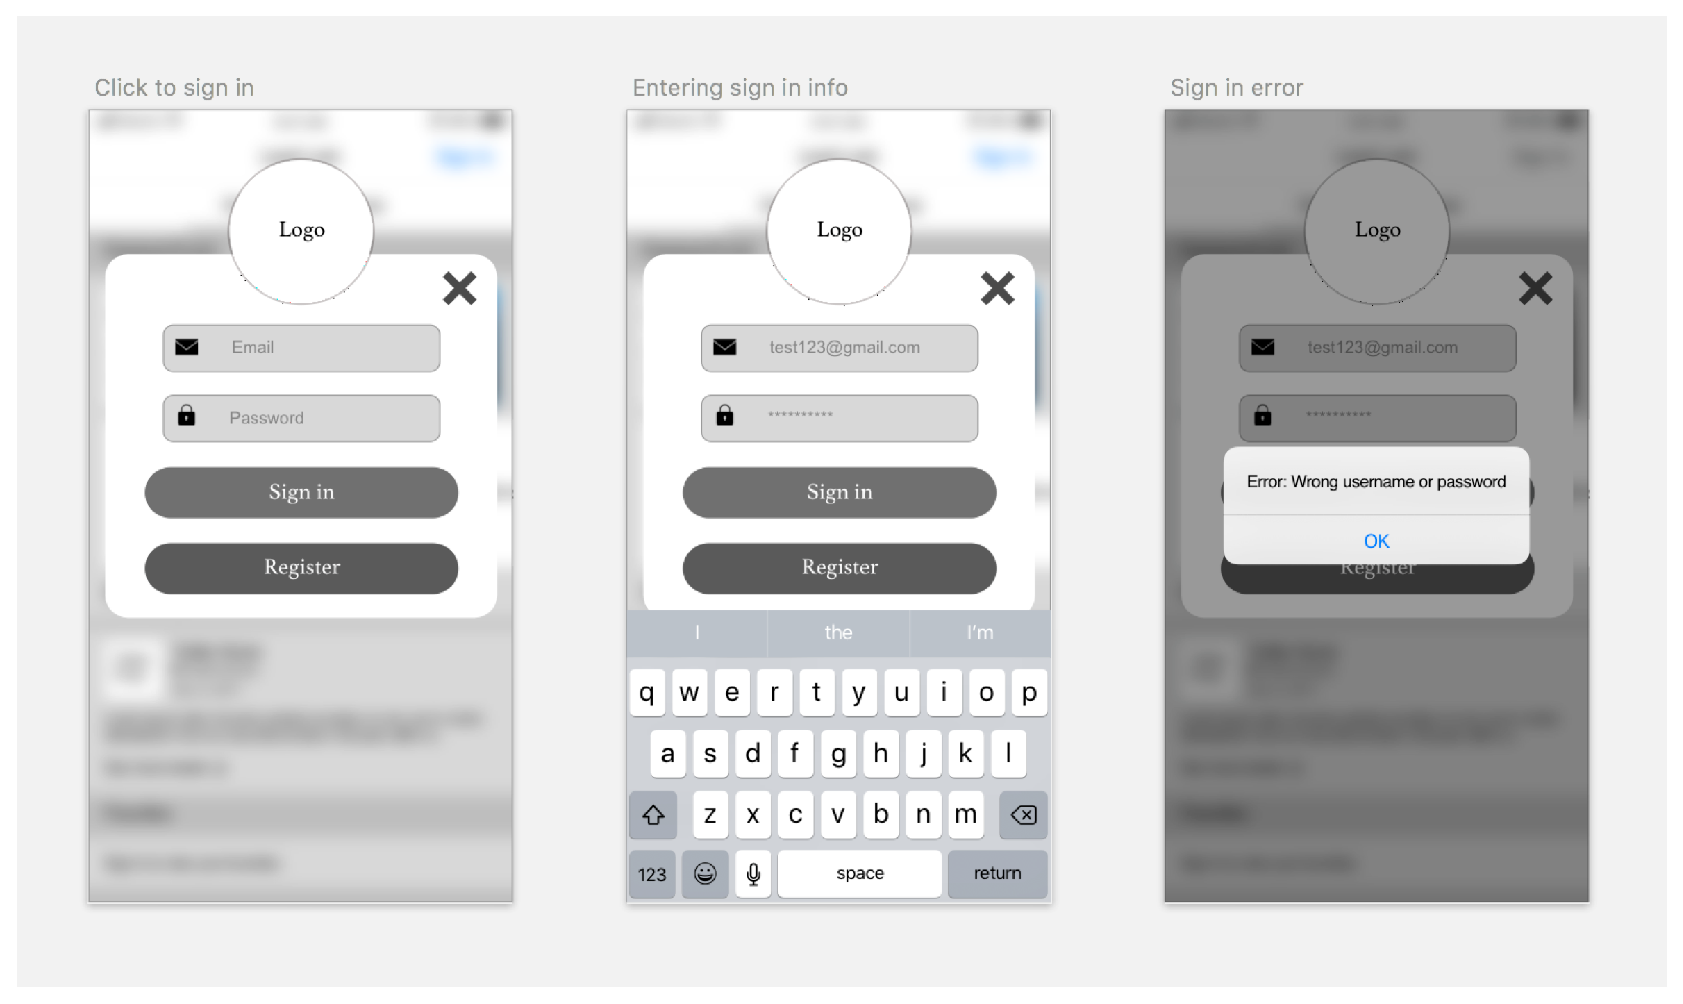
\includegraphics[scale=.50]{SignIn}
\caption{Register User Interface}
\captionsetup{justification=centering}
\end{figure}

\begin{figure}[H]
\centering
\captionsetup{justification=centering}
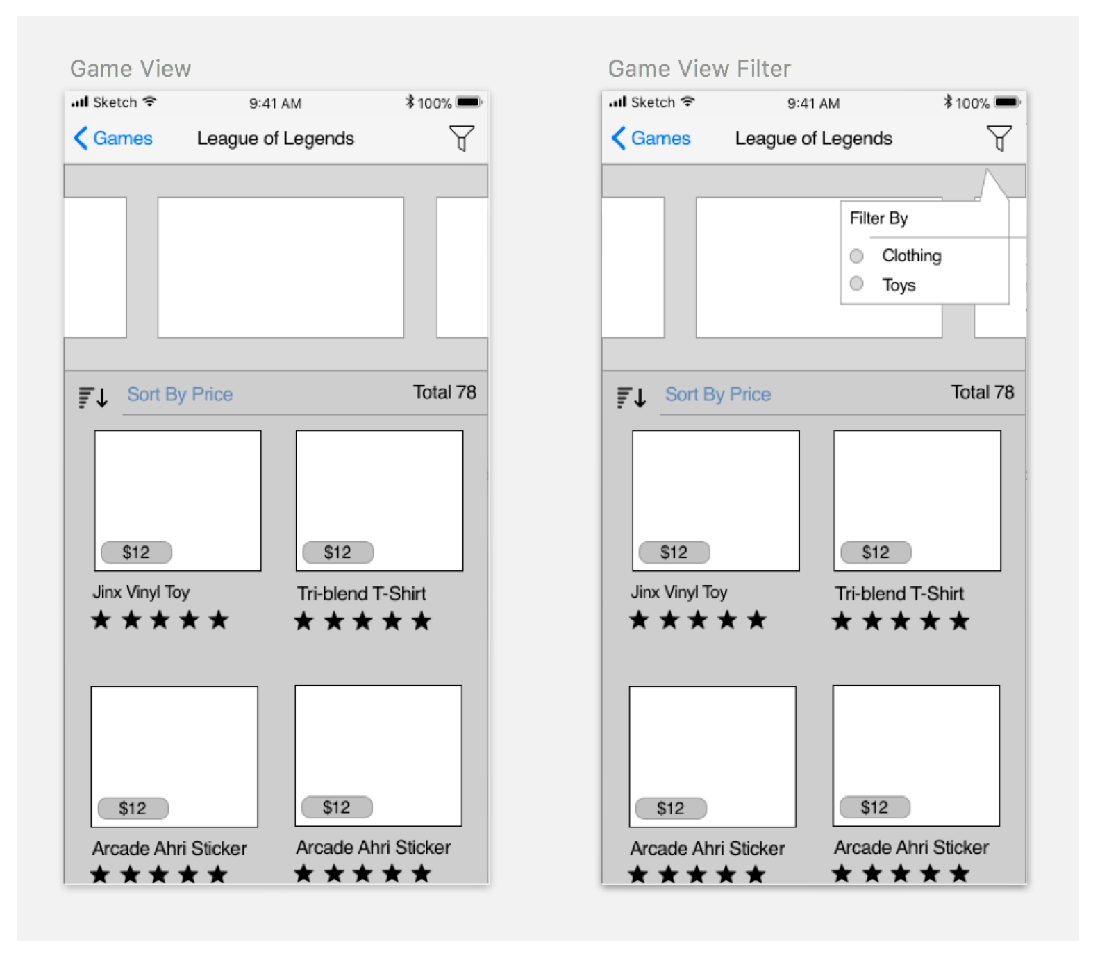
\includegraphics[scale=.50]{GameView}
\caption{Game View User Interface}
\captionsetup{justification=centering}
\end{figure}

\bibliographystyle{IEEEtran}
\bibliography{design_doc}

\end{document}